\documentclass[12pt, letterpaper]{article}
\usepackage[spanish]{babel}
\usepackage[utf8]{inputenc}
\usepackage{graphicx}
\usepackage{amssymb}
\graphicspath{{./imagenes/}}
\usepackage{xcolor}

%Paquetes para símbolos y entornos matematicos. En este documento se usa para poder usar el tag \begin{align} y \begin{align*} que permiten alinear expresiones matemáticas
\usepackage{amsmath}
\usepackage{amssymb}
%paquete que permite el uso de del argumento H al momento de insertar imágenes
\usepackage{float}

%comando para especificar el título del documento 
\title{Matemáticas para las Ciencias Aplicadas I}

%comando para especificar el autor del documento
\author{Pérez Romero Natalia Abigail}

%comando para especificar la fecha del documento
\date{\today}
%--------------Fin preámbulo--------------

%------------Inicio documento-------------
\begin{document}
%comando que genera el titulo con los datos especificados en el preámbulo
\maketitle
\textbf{Tarea VIII. Ejercicios del libro Cálculo. Una variable de Thomas J.R, George B.}

\textbf{Ejercicios 1, 2, 3, 5 y 6 de la sección 2.1 Razón de Cambios y Límites.}

Determine los límites que se piden para la función $g(x)$, cuya gráfica se muestre a continuación, o explique porqué no existen.
\begin{figure}[ht]
\centering
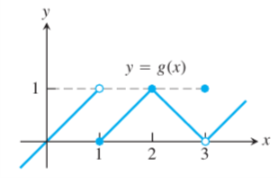
\includegraphics[width=20em]{t8uno}
\end{figure}

\textbf{a)} \[ \lim_{x \to 1} g(x)\]

Al observar la gráfica notó que cuando nos acercamos a $x = 1$  por la derecha $g(x)$ tiende a 0\\
Y cuando nos acercamos a $x = 1$ por la izquierda $g(x)$ tiende a 1
El límite de una función no puede acercarse a dos valores, por lo que decimos que el límite no existe cuando $x \to 1$

\textbf{b)} \[ \lim_{x \to 2} g(x)\]

Al observar la gráfica notó que cuando nos acercamos a $x = 2$  por la derecha $g(x)$ tiende a 1\\
Y cuando nos acercamos a $x = 2$ por la izquierda $g(x)$ tiende a 1

Por lo que \[ \lim_{x \to 2} g(x) = 1\]

\textbf{b)} \[ \lim_{x \to 3} g(x)\]

Al observar la gráfica notó cuando nos acercamos a $x = 3$  por la derecha $g(x)$ tiende a 0\\
Y cuando nos acercamos a $x = 3$ por la izquierda $g(x)$ tiende a 0\\

Por lo que \[ \lim_{x \to 3} g(x) = 0\]

\textbf{Encuentre los límites que se piden para la función $f(t)$, cuya gráfica se muestre a continuación, o explique porqué no existen.}

\begin{figure}[ht]
\centering
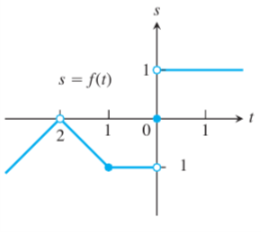
\includegraphics[width=20em]{t8dos}
\end{figure}

\textbf{a.} \[ \lim_{t \to -2} f(t)\]
Al observar la gráfica notó cuando nos acercamos a $x = -2$  por la derecha $f(t)$ tiende a 0\\
Y cuando nos acercamos a $x = -2$ por la izquierda $f(t)$ tiende a 0\\
Por lo que \[ \lim_{t \to -2} f(t) = 0\]


\textbf{b.} \[ \lim_{t \to -1} f(t)\]

Al observar la gráfica notó cuando nos acercamos a $x = -1$  por la derecha $f(t)$ tiende a -1\\
Y cuando nos acercamos a $x = -1$ por la izquierda $f(t)$ tiende a -1\\
Por lo que \[ \lim_{t \to -1} f(t) = -1\]

\textbf{c.} \[ \lim_{t \to 0} f(t)\]

Al observar la gráfica notó cuando nos acercamos a $x = 0$  por la derecha $f(t)$ tiende a 1\\
Y cuando nos acercamos a $x = 0$ por la izquierda $f(t)$ tiende a -1\\

El límite de una función no puede acercarse a dos valores, por lo que decimos que el límite no existe cuando $x \to 0$

\newpage 
\textbf{¿Cuáles de las afimaciones siguientes acerca de la función $y = f(x)$, cuya gráfica se muestra a continuación, son ciertas y cuáles son falsas}

\begin{figure}[ht]
\centering
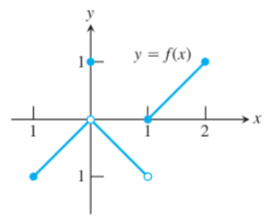
\includegraphics[width=20em]{t8tres}
\end{figure}

\textbf{a.} $\lim_{x \to 0} f(x)$ existe \\
Es verdad, porque cuando nos acercamos a $x = 0$  por la derecha $f(t)$ tiende a 0\\
Y cuando nos acercamos a $x = 0$ por la izquierda $f(t)$ tiende a 0

\textbf{b.} \[ \lim_{x \to 0} f(x) = 0\]
Es verdad, porque  a pesar de que  $f(x)$ esté definida para $x = 0$, es decir $f(0)= 1$, el límite de manera intuitiva se entiende como lo que sucede con la función cuando se  'acerca' a cierta $x$, En \textbf{a.} se obtuvo con los límites laterales  que $\lim_{x \to 0} f(x) = 0$

\textbf{c.} \[ \lim_{x \to 0} f(x) = 1\]
Es falso, porque  a pesar de que  $f(x)$ esté definida para $x = 0$, es decir $f(0)= 1$, el límite de manera intuitiva se entiende como lo que sucede con la función cuando se  'acerca' a cierta $x$, y como en \textbf{a.} se obtuvo con los límites laterales que $\lim_{x \to 0} f(x) = 0$, así que $\lim_{x \to 0} f(x) = 1$   es falso.

\textbf{d.} \[ \lim_{x \to 1} f(x) = 1\]

Es falso, porque cuando nos acercamos a $x = 1$  por la derecha $f(x)$ tiende a 0\\
Y cuando nos acercamos a $x = 1$ por la izquierda $f(x)$ tiende a -1. Lo que quiere decir que no existe el límite cuando $x \to 1$

\textbf{e.}  \[ \lim_{x \to 1} f(x) = 0\]
Es falso, porque  a pesar de que  $f(x)$ esté definida para $x = 1$, es decir $f(1)= 0$, el límite de manera intuitiva se entiende como lo que sucede con la función cuando se  'acerca' a cierta $x$, pero en \textbf{d.} observamos que no existe el límite cuando $x \to 1$

\textbf{f.} $\lim_{x \to x_0} f(x)$ existe en cualquier punto $x_0$ en $(-1,1)$

Es verdad, porque en el intervalo abierto $(-1,1)$ (no se incluye $x = 1$) observamos que no hay segmentos de gráfica que se aproximen a una misma $x$ 

\textbf{Existencia de límites. En los siguientes ejercicios explique por qué no existen los límites}

\textbf{5.} \[ \lim_{x \to 0} \frac{x}{|x|}\]

\begin{figure}[ht]
\centering
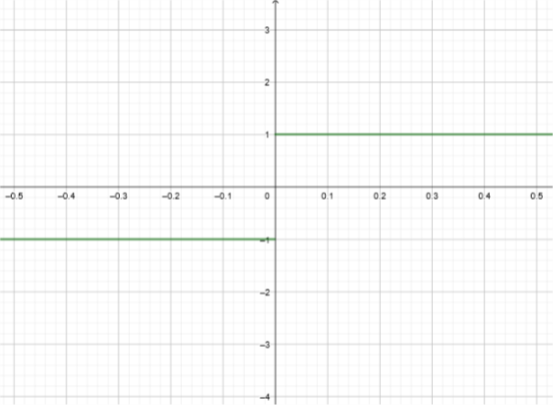
\includegraphics[width=20em]{t8cuatro}
\end{figure}

No existe el límite, la función es continua excepto cuando $x = 0$, y cuando  $x \to 0$, la función tiende por la derecha a 1, y tiende por la izquierda a -1, el límite no puede tender a más de un valor.

\textbf{6.} \[ \lim_{x \to 1} \frac{1}{x - 1}\]

\begin{figure}[ht]
\centering
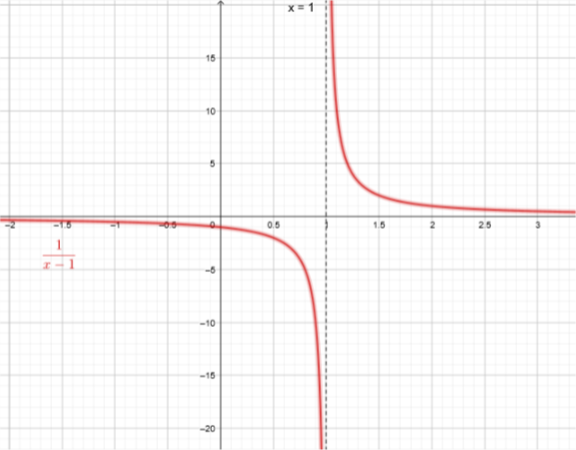
\includegraphics[width=20em]{t8cinco}
\end{figure}

No existe el límite, porque la función es continua excepto cuando $x = 1$, y cuando  $x \to 0$, la función tiende por la derecha a $\infty$ , y tiende por la izquierda a $-\infty$.
\end{document}